\subsubsection{$H \to \gamma\gamma$}
\label{sec:Hgammagamma}
%% {\it To be written by: M. Delmastro}

The measurement of the Higgs boson properties in the \Hyy\ channel is performed using the events that contain two isolated photon candidates passing good quality requirements in the precision regions of the detectors. Events are further segmented according to the objects accompanying the diphoton system, in order to maximize the sensitivity to the main Higgs production modes and to reduce the uncertainties on the respective cross sections, as well as to the Simplified Template Cross Section (STXS, first introduced in Refs. \cite{deFlorian:2016spz,Badger:2016bpw}) in the merged version of Stage-1.
The Higgs production cross sections are measured for a Higgs boson absolute rapidity $|y_H|$ smaller than 2.5, and with further requirements on the objects accompanying the diphoton system (e.g. jet $p_\mathrm{T}$).
%%
The \Hyy\ signal is extracted by means of a combined signal-plus-background fit of the diphoton invariant mass spectra in the various event categories, where both the continuous background and the signal resonance are parameterized by analytical functions. The shape properties of the signal PDF are obtained by Monte Carlo (MC) simulation, and constrained by performance studies of the photon energy scale and resolution. The background PDF is completely determined by the fit on data, with systematic uncertainties attributed to the specific choice of functional form following the procedure described in Ref. \cite{Aad:2012tfa} or using the discrete profiling method \cite{Dauncey:2014xga}. More details on the analyses methods can be found in most recent measurements in the \Hyy\ channel published by ATLAS \cite{ATLAS:2018uso} and CMS \cite{Sirunyan:2018ouh}. 

The performance of the measurement of the Higgs boson properties in the \Hyy\ channel at HL-LHC is extrapolated from the most recent measurements by ATLAS with 80\,$\mathrm{fb}^{-1}$ \cite{ATLAS:2018uso} and by CMS with 36\,$\mathrm{fb}^{-1}$ \cite{Sirunyan:2018ouh}. The main systematic uncertainties affecting the results are the background modelling uncertainty,
%% QCD scale uncertainties
missing higher order uncertainties
causing event migrations between the bins, photon isolation efficiencies and jet uncertainties.
%% Beside that, the underlying event and parton showering uncertainties as well as the PES and PER play are role.
%
On top of the common assumptions mentioned in Section~\ref{sec:HiggsExtrapAss}, the %ATLAS \Hyy\ 
results of the studies perfromed by ATLAS include a 10\% increase of the background modeling systematic uncertainties, to account for the potentially worst knowledge of the background composition in each analysis category at HL-LHC: this assumption has anyway negligible impact.
%
In the Run-2 analyses, a conservative 100\% uncertainty on the heavy flavour resonant background in top-sensitive categories is applied. Measurements by ATLAS and CMS of the heavy flavour content, or the $b$-jet multiplicity, are expected to better constrain these contributions: for the S2 scenario extrapolation, this uncertainty is therefore halved.

Figure~\ref{fig:Hyy_ATLAS_HLLHC_S2} shows the ratio of the extrapolated \Hyy\ ATLAS measurements of the cross sections times branching fraction of the main Higgs production modes to their respective theoretical SM predictions (left), and uncertainties on these measurements for S1, S2, and stat-only scenarios as extrapolated using the \Hyy\ CMS measurements (right). CMS extrapolation is obtained from the simultaneous fit in all production and decay modes, as described in Section \ref{sec:expcomb_prodtimesdecay}. The reduction of the total uncertainty with respect to the 80\,$\mathrm{fb}^{-1}$ results ranges from a factor of about 2 (3) for the S1 (S2) scenario for the $ggH+b\bar{b}H$, VBF, top cross sections, to a factor of about 5(6) for the $VH$ cross section, that remains dominated by the statistical uncertainty.

\begin{figure}
  \centering
  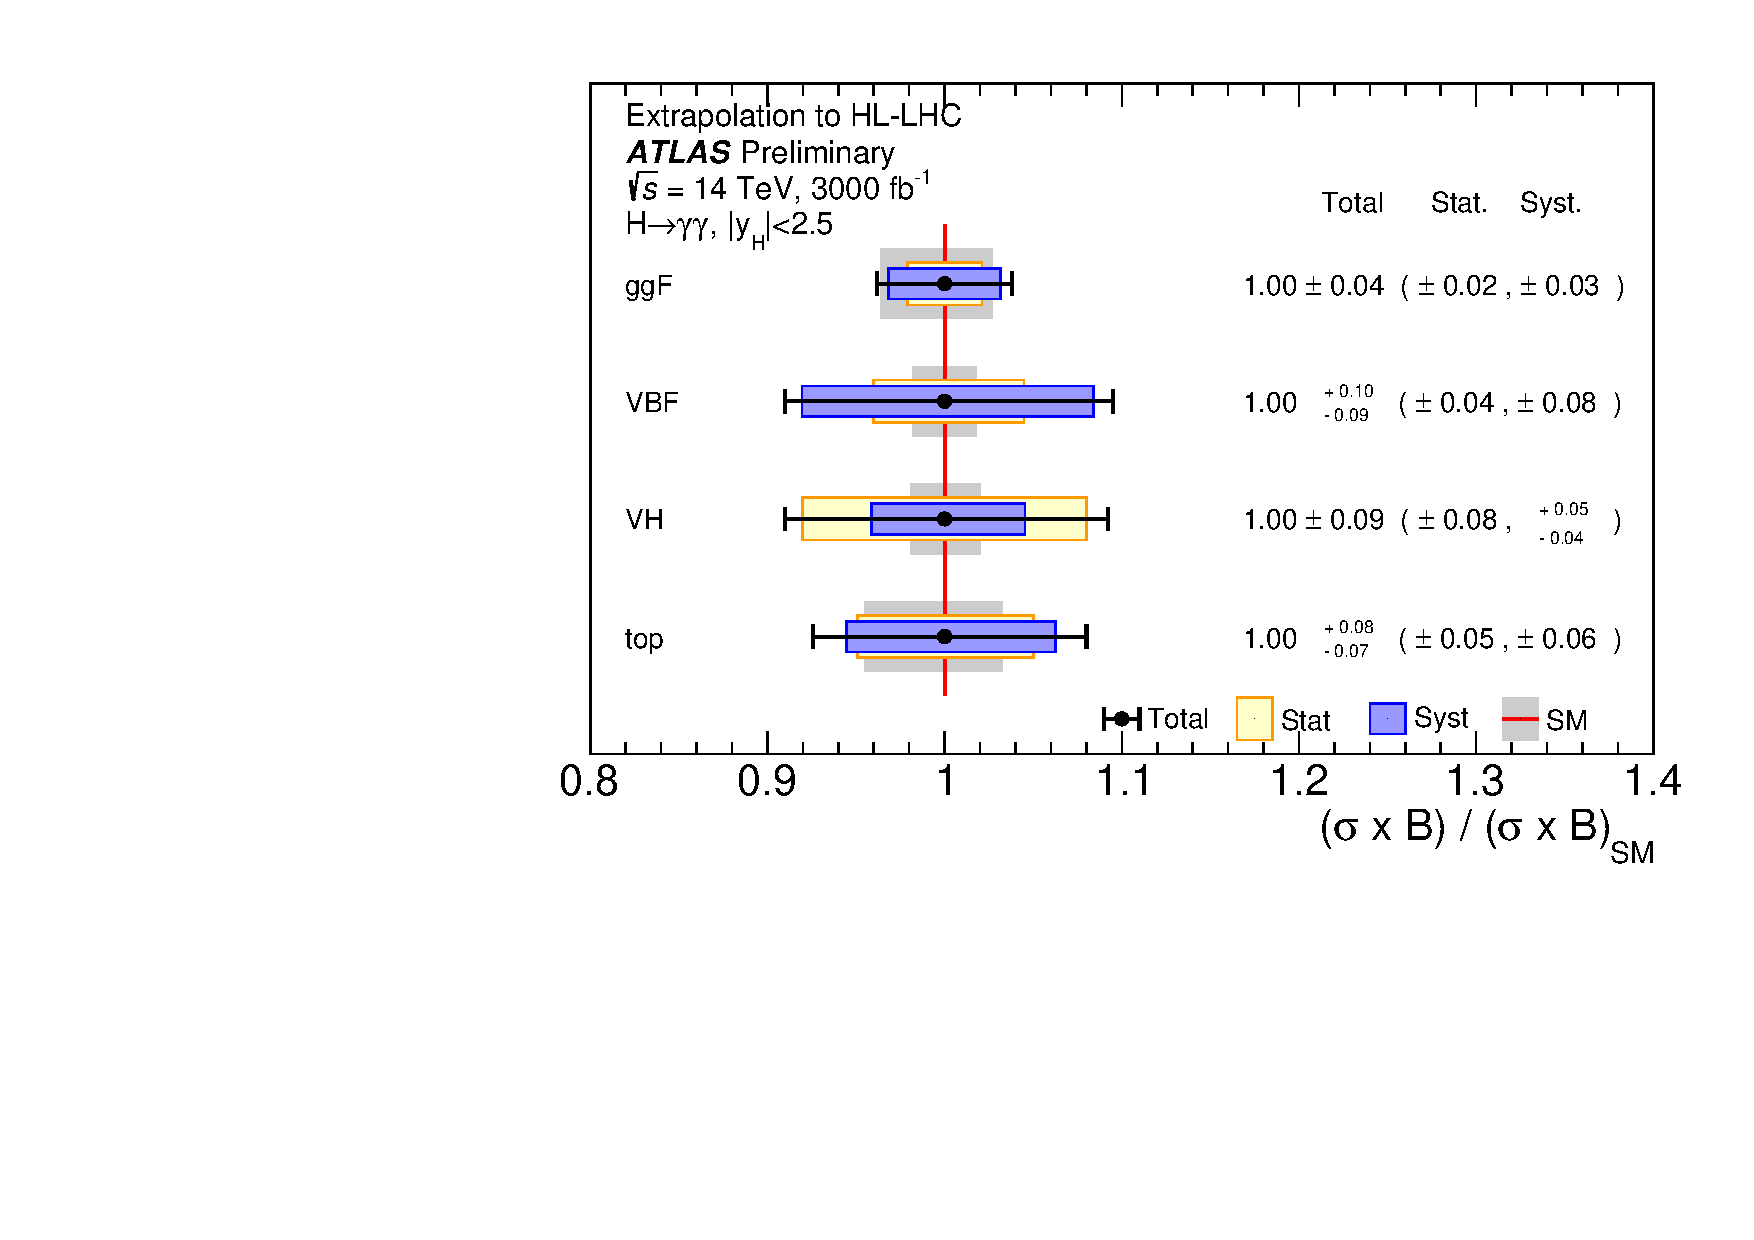
\includegraphics[width=0.56\linewidth]{\main/section2/plots/channels/ATLAS_plot_compareToSM_yy_prodXS}
  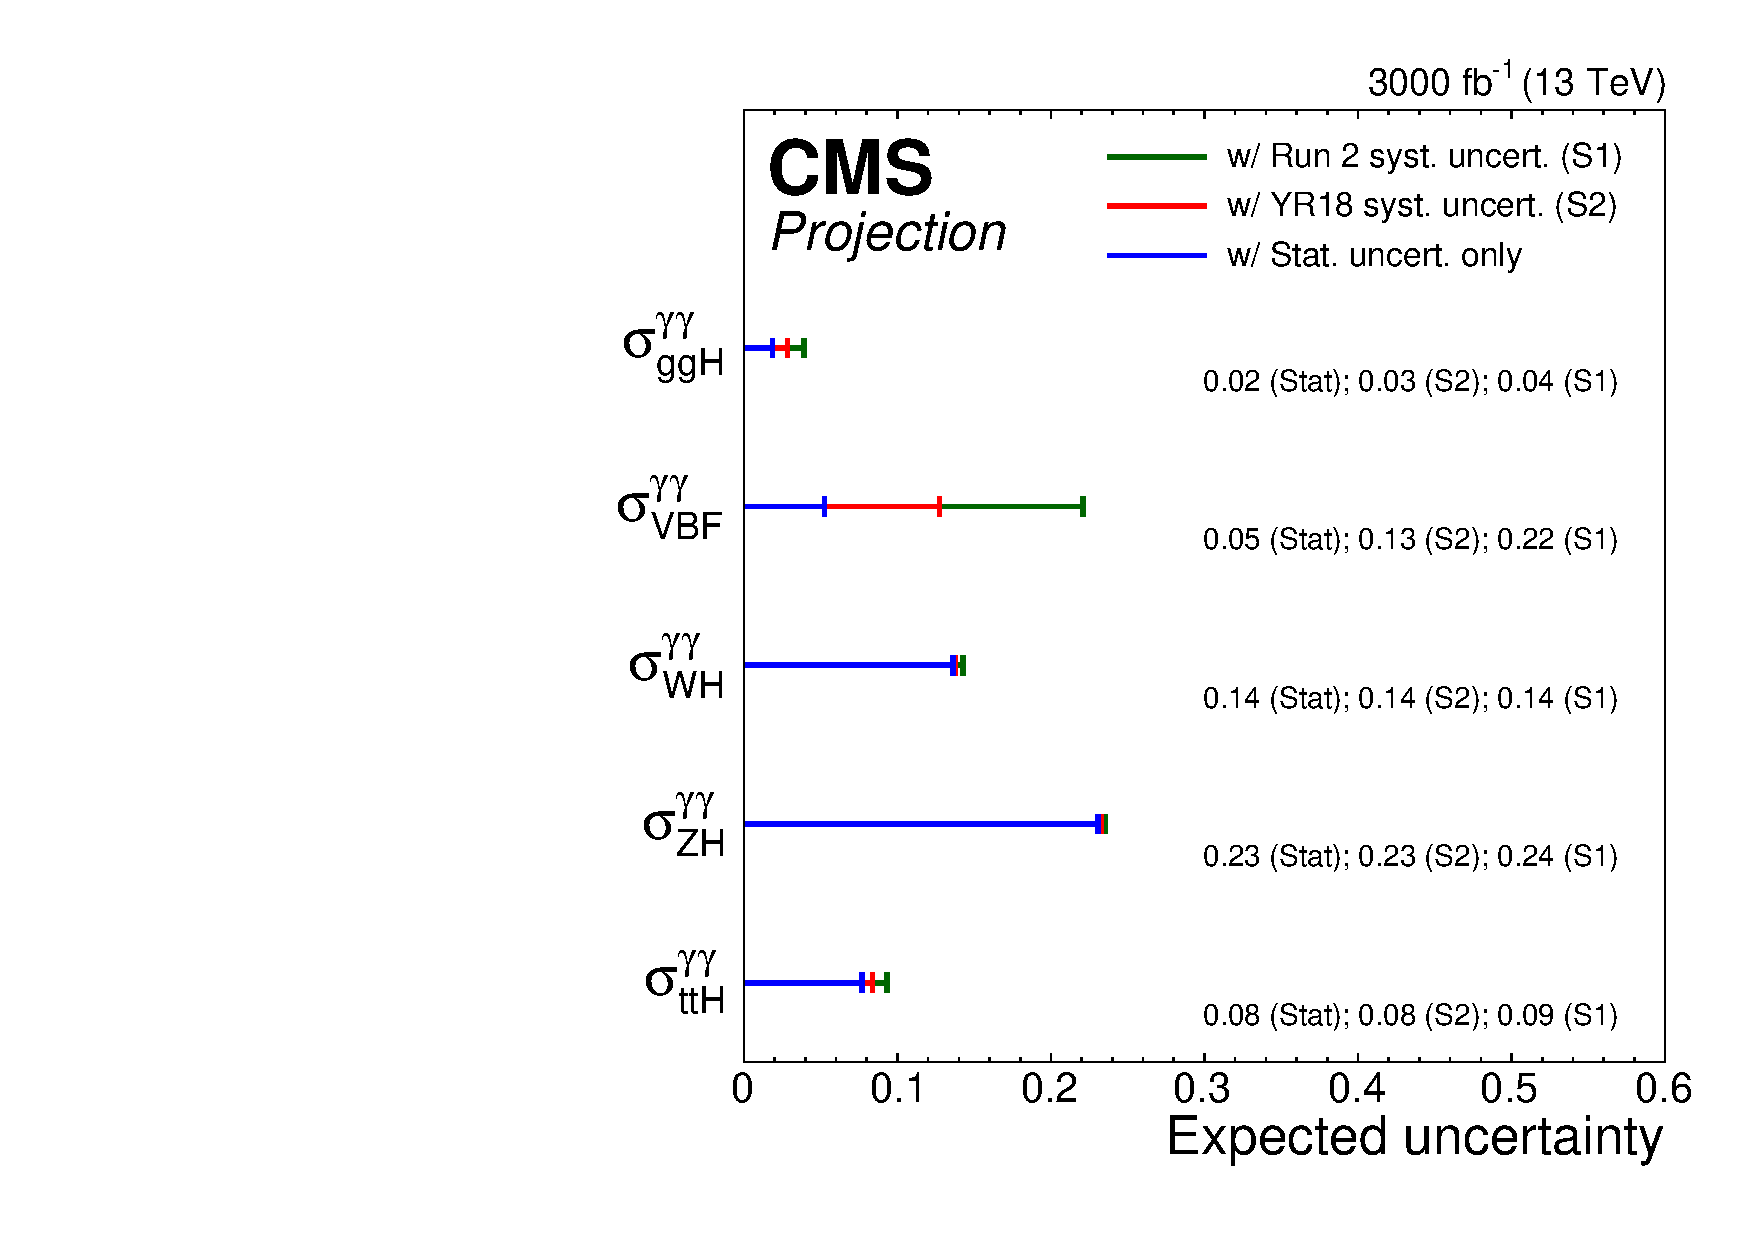
\includegraphics[width=0.42\linewidth]{\main/section2/plots/channels/CMS_summary_A1_5PD_3000_hgg}
  \caption{Cross-section times branching fraction measurements of the main Higgs production modes in the \Hyy\ decay channel, as extrapolated at the HL-LHC. In case of ATLAS results (left) the ratios of cross sections to their respective theoretical SM predictions are shown for scenario S2, while in case of CMS results (right) the uncertainties on these measurements are shown for S1, S2, and Stat-only scenarios..}
  \label{fig:Hyy_ATLAS_HLLHC_S2}
\end{figure}

\subsubsection{$H \to Z\gamma \to \ell\ell\,\gamma$}
%%{\it To be written by: M. Delmastro}

Due to the small branching fraction in the SM, the \HZy\ decay has not yet been observed at the LHC. The experimental observed limits at the $95\%$ confidence level are currently 6.6 times the SM prediction for a Higgs boson mass of 125.09 GeV by ATLAS and 3.9 times the SM prediction for a Higgs boson mass of 125 GeV by CMS, based on the analyses of 36\,$\mathrm{fb}^{-1}$ of $pp$ collision at $\sqrt{s} = 13$ TeV described in Ref. \cite{Aaboud:2017uhw, Sirunyan:2018tbk}.

The analyses select events with an isolated photon candidate passing good quality requirements in the precision regions of the detectors, and a dilepton system with properties compatible with that of the decay of a $Z$ boson. Events are separated according to lepton flavour, the event kinematic properties, and the presence of jets compatible with the VBF production of the Higgs boson, in order to maximize the signal sensitivity. The signal is sought for by means of a combined signal-plus-background fit of the photon-dilepton invariant mass spectra in various event categories, where both the continuous background and the signal resonance are parameterized by analytical functions. The Run-2 analyses are strongly driven by statistical uncertainty, and the main systematic uncertainties are from the bias associated to the background modeling.

The extrapolations to HL-LHC are performed with a simple scaling approach, assuming the same signal and background modeling used in the Run-2 analyses. All experimental and systematic uncertainties are considered to remain the same (S1), except the uncertainty associated to the background modeling, which is taken to be negligible.

The ATLAS expected significance to the SM Higgs boson decaying in $Z\gamma$ is 4.9 $\sigma$ with 3000\,$\mathrm{fb}^{-1}$. Assuming the SM Higgs production cross section and decay branching ratios, the signal strength is expected to be measured with a $\pm0.24$ uncertainty. The cross section times branching ratio for the $pp\rightarrow H \rightarrow Z\gamma$ process is projected to be measured as $1.00\pm0.23$ times the SM prediction. Even at the HL-LHC scenario S1, the analysis sensitivity  to \HZy\ will remain driven by the statistical uncertainty. The dominant source of systematic uncertainty in the extrapolation is that associated to the 
%% QCD scale variations.
missing higher order uncertainties.

\subsubsection{$H \to ZZ^* \to 4\ell$}
%% {\it To be written by: M. Delmastro}

The measurement of the Higgs boson properties in the \HZZ\ channel is performed using the events that contain at least two same-flavour opposite-sign dilepton pairs, chosen from isolated electrons and muons candidates passing good quality requirements in the precision regions of the detectors. Additional constraints on the kinematical properties of the lepton pair associated with the decay of the on-shell $Z$ boson, and on the global topology of the event, helps to improve the signal to background ratio. The four-lepton invariant mass resolution is improved by correcting for the emission of final-state radiation photons by the leptons.
%%
The \HZZ\ signal is extracted from the four-lepton invariant mass spectra in the different event categories, after having evaluated the background components using simulations to constrain their shapes, and data control regions to extrapolate their normalization in the signal regions. Signal to background sensitivity is in general enhanced using the multivariate and/or matrix-element based techniques. More details on the analyses methods can be found in most recent measurements in the \HZZ\ channel published by ATLAS \cite{ATLAS:2018bsg} and CMS \cite{Sirunyan:2017exp}.

The performance of the measurement of the Higgs boson properties in the \HZZ\ at HL-LHC is extrapolated from the most recent measurements by ATLAS with 80\,$\mathrm{fb}^{-1}$ \cite{ATLAS:2018bsg}, and by CMS with 36\,$\mathrm{fb}^{-1}$ \cite{Sirunyan:2017exp}.
CMS extrapolation is obtained from the simultaneous fit in all production and decay modes, as described in Section \ref{sec:expcomb_prodtimesdecay}.
The dominant systematic uncertainties affecting the extrapolation of the ggH cross section measurement are the lepton reconstruction and identification efficiencies, and pile-up modeling uncertainties. The VBF and VH cross-sections are primarily affected by the uncertainty on the jet energy scale and resolution, and by the
%% QCD scale uncertainties.
missing higher order uncertainties.
These and
%% The theory uncertainties related to QCD scale
the parton shower modeling primarily affects the extrapolated top cross section.

The VBF, VH and especially top measurements in the \HZZ\ decay channel remain largely dominated by statistical uncertainty when extrapolated to 3000\,$\mathrm{fb}^{-1}$ while the $ggH+b\bar{b}H$ cross section is dominated by systematic uncertainties both in scenario S1 and S2.
%
Figure~\ref{fig:HZZ_ATLAS_HLLHC_S2} shows the ratio of the extrapolated \HZZ\ ATLAS measurements of the main Higgs boson production modes to their respective theoretical SM predictions in the scenario S2 (left), and uncertainties on these measurements for S1, S2, and stat-only scenarios as extrapolated using the \HZZ\ CMS measurements (right). The ggF and top \HZZ\ measurements at HL-LHC are expected to reach a level of precision comparable to the projected uncertainty on the corresponding theory predictions.

\begin{figure}
  \centering
  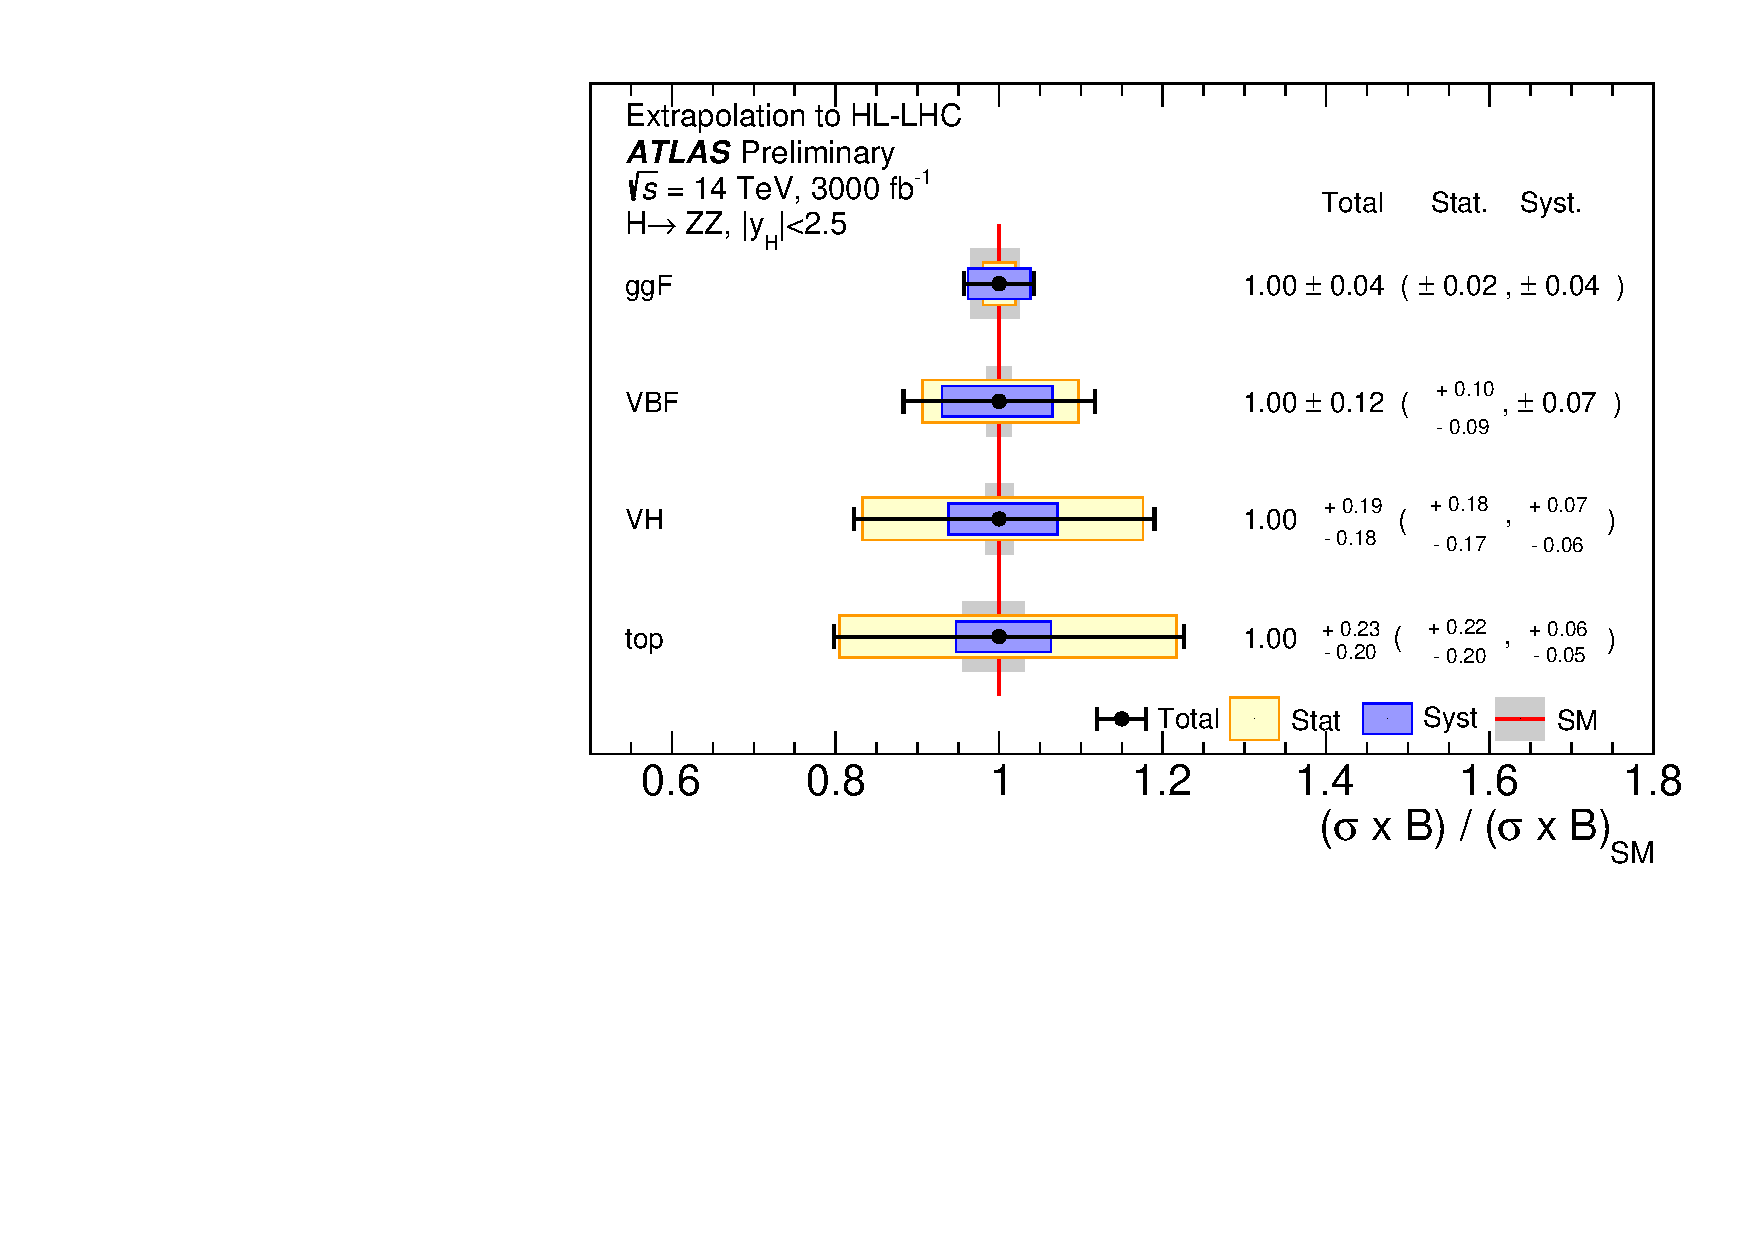
\includegraphics[width=0.56\linewidth]{\main/section2/plots/channels/ATLAS_plot_compareToSM_ZZ_prodXS}
  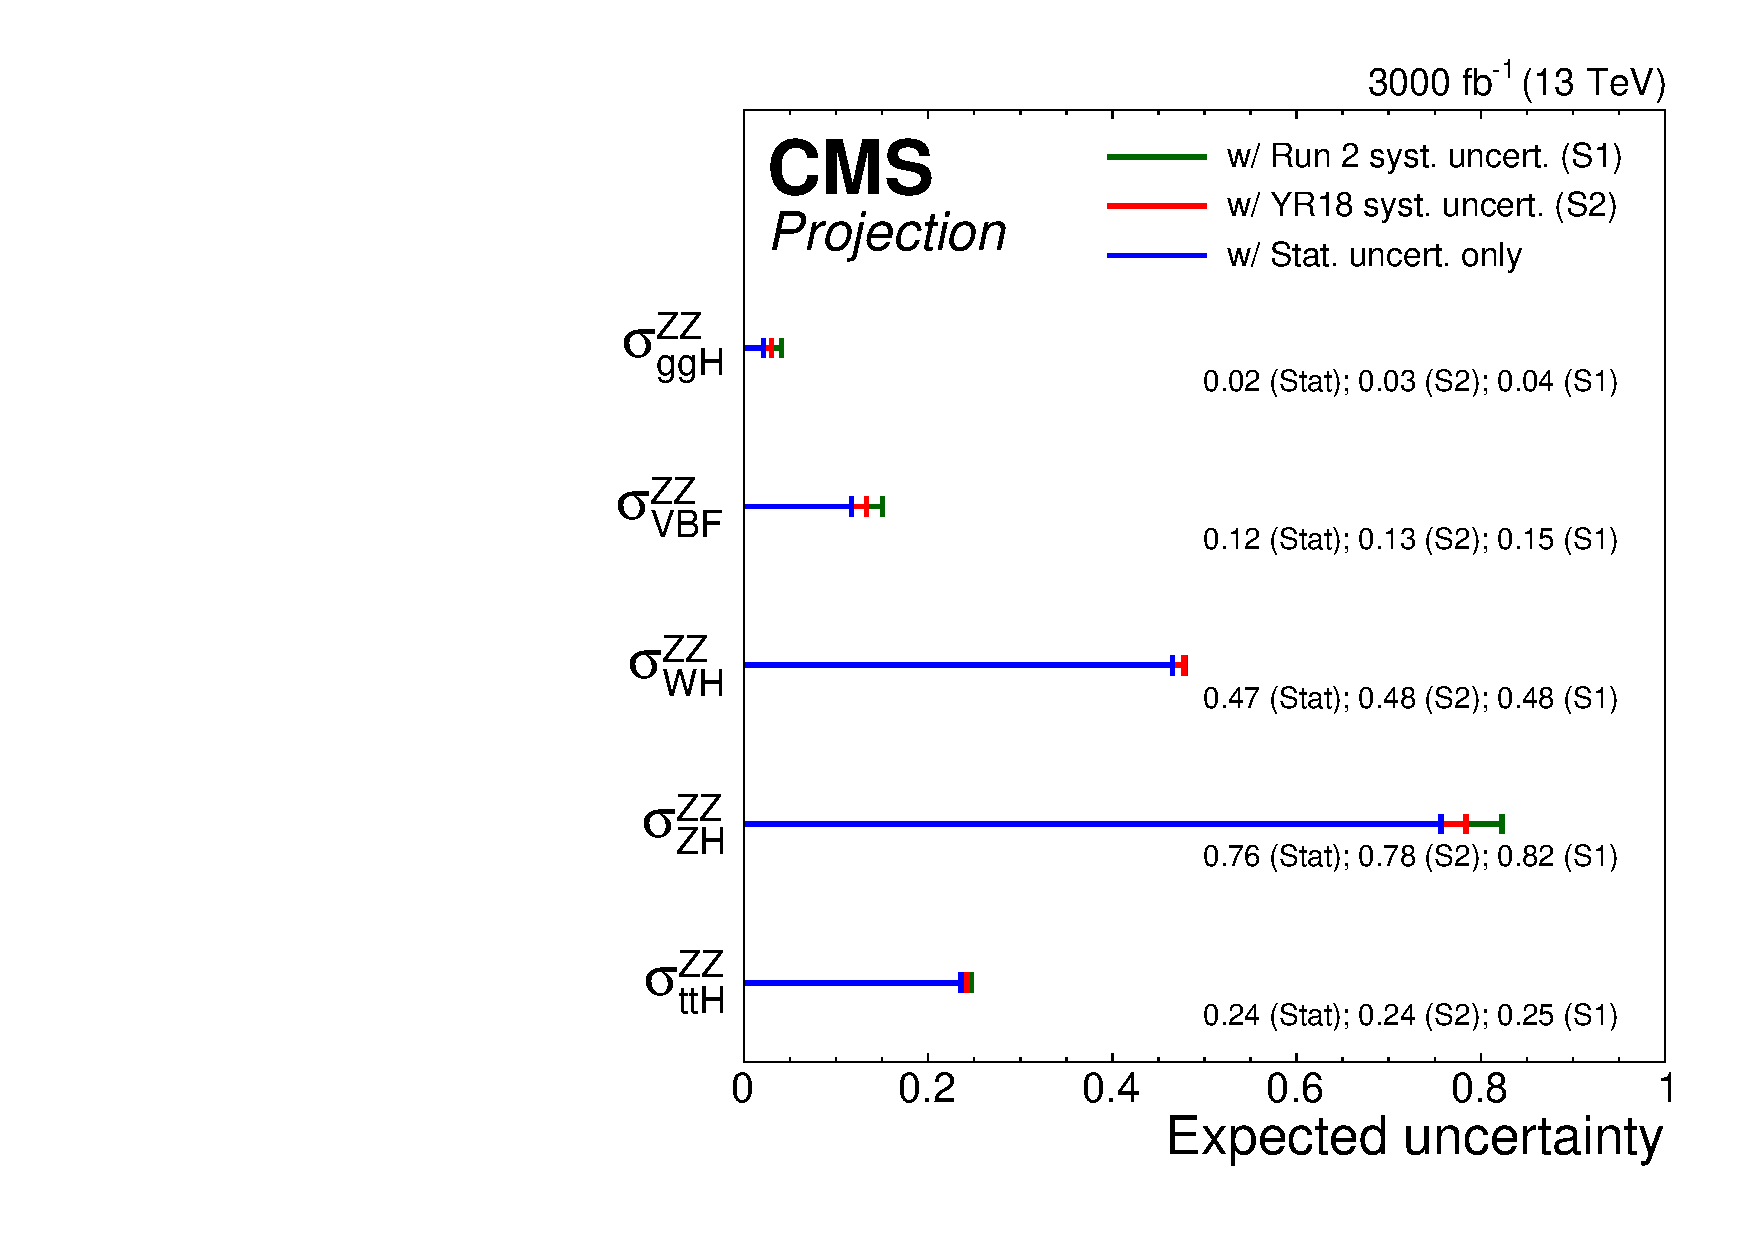
\includegraphics[width=0.42\linewidth]{\main/section2/plots/channels/CMS_summary_A1_5PD_3000_hzz}
  \caption{Cross-section times branching fraction measurements of the main Higgs boson production modes in the \HZZ\ decay channel, as extrapolated at the HL-LHC. In case of ATLAS results (left) the ratios of cross sections to their respective theoretical SM predictions are shown for scenario S2, while in case of CMS results (right) the uncertainties on these measurements are shown for S1, S2, and Stat-only scenarios.}
  \label{fig:HZZ_ATLAS_HLLHC_S2}
\end{figure}

\subsubsection{$H \to WW^* \to \ell\nu\,\ell\nu$}
%% {\it To be written by: M. Delmastro}

The measurement of the Higgs boson properties in the \HWW\ channel is performed using the events that contain two opposite-charged isolated leptons passing good quality requirements in the precision region of the detectors and missing transverse momentum. Additional requirements on the event kinematical properties are applied to reduce the various background components (e.g. requirements on the dilepton invariant mass, transverse mass of the di-lepton + missing-transverse-energy (MET) system). Events are categorized as a function of the jet multiplicity in order to exploit the different background composition in different categories, and to help extracting the Higgs ggH and VBF production cross sections. The normalizations of the top ($t\bar{t}$ and $W+t$), and $Z\rightarrow\tau\tau$ backgrounds are set using dedicated control regions of the same jet multiplicity as the signal category to which the normalization is transferred. In case of the (non-resonant) $WW$ background, its normalization is either determined using dedicated control regions (ATLAS approach) or by using theoretical prediction with corresponding uncertainty on it (CMS approach). More details on the analyses methods can be found in most recent measurements in the \HWW\ channel published by ATLAS \cite{Aaboud:2018jqu} and CMS \cite{Sirunyan:2018egh}.

The performance of the measurements of Higgs boson properties in the \HWW\ channel at HL-LHC is extrapolated from the most recent measurements in this channel performed by ATLAS with 80\,$\mathrm{fb}^{-1}$ \cite{Aaboud:2018jqu} and by CMS with 36\,$\mathrm{fb}^{-1}$ \cite{Sirunyan:2018egh}. These measurements are completely dominated by systematic uncertainties, and their extrapolation to the S2 scenario shows the expected reduction by a factor two. The measurement of the ggH cross section by branching fraction is dominated by theoretical PDF uncertainty, followed by experimental uncertainties affecting the signal acceptance, including uncertainties on the jet energy scale and flavour composition, and lepton misidentification; the VBF result suffers from similar dominant uncertainties.
%%
Figure~\ref{fig:HWW_ATLAS_HLLHC_S2} shows the ratio of the extrapolated \HWW\ ATLAS measurements of the main Higgs production modes to their respective theoretical SM predictions in scenario S2 (left), and uncertainties on these measurements for S1, S2, and Stat-only scenarios as extrapolated using the \HWW\ CMS measurements (right). CMS extrapolation is obtained from the simultaneous fit in all production and decay modes, as described in Section \ref{sec:expcomb_prodtimesdecay}.

\begin{figure}
  \centering
  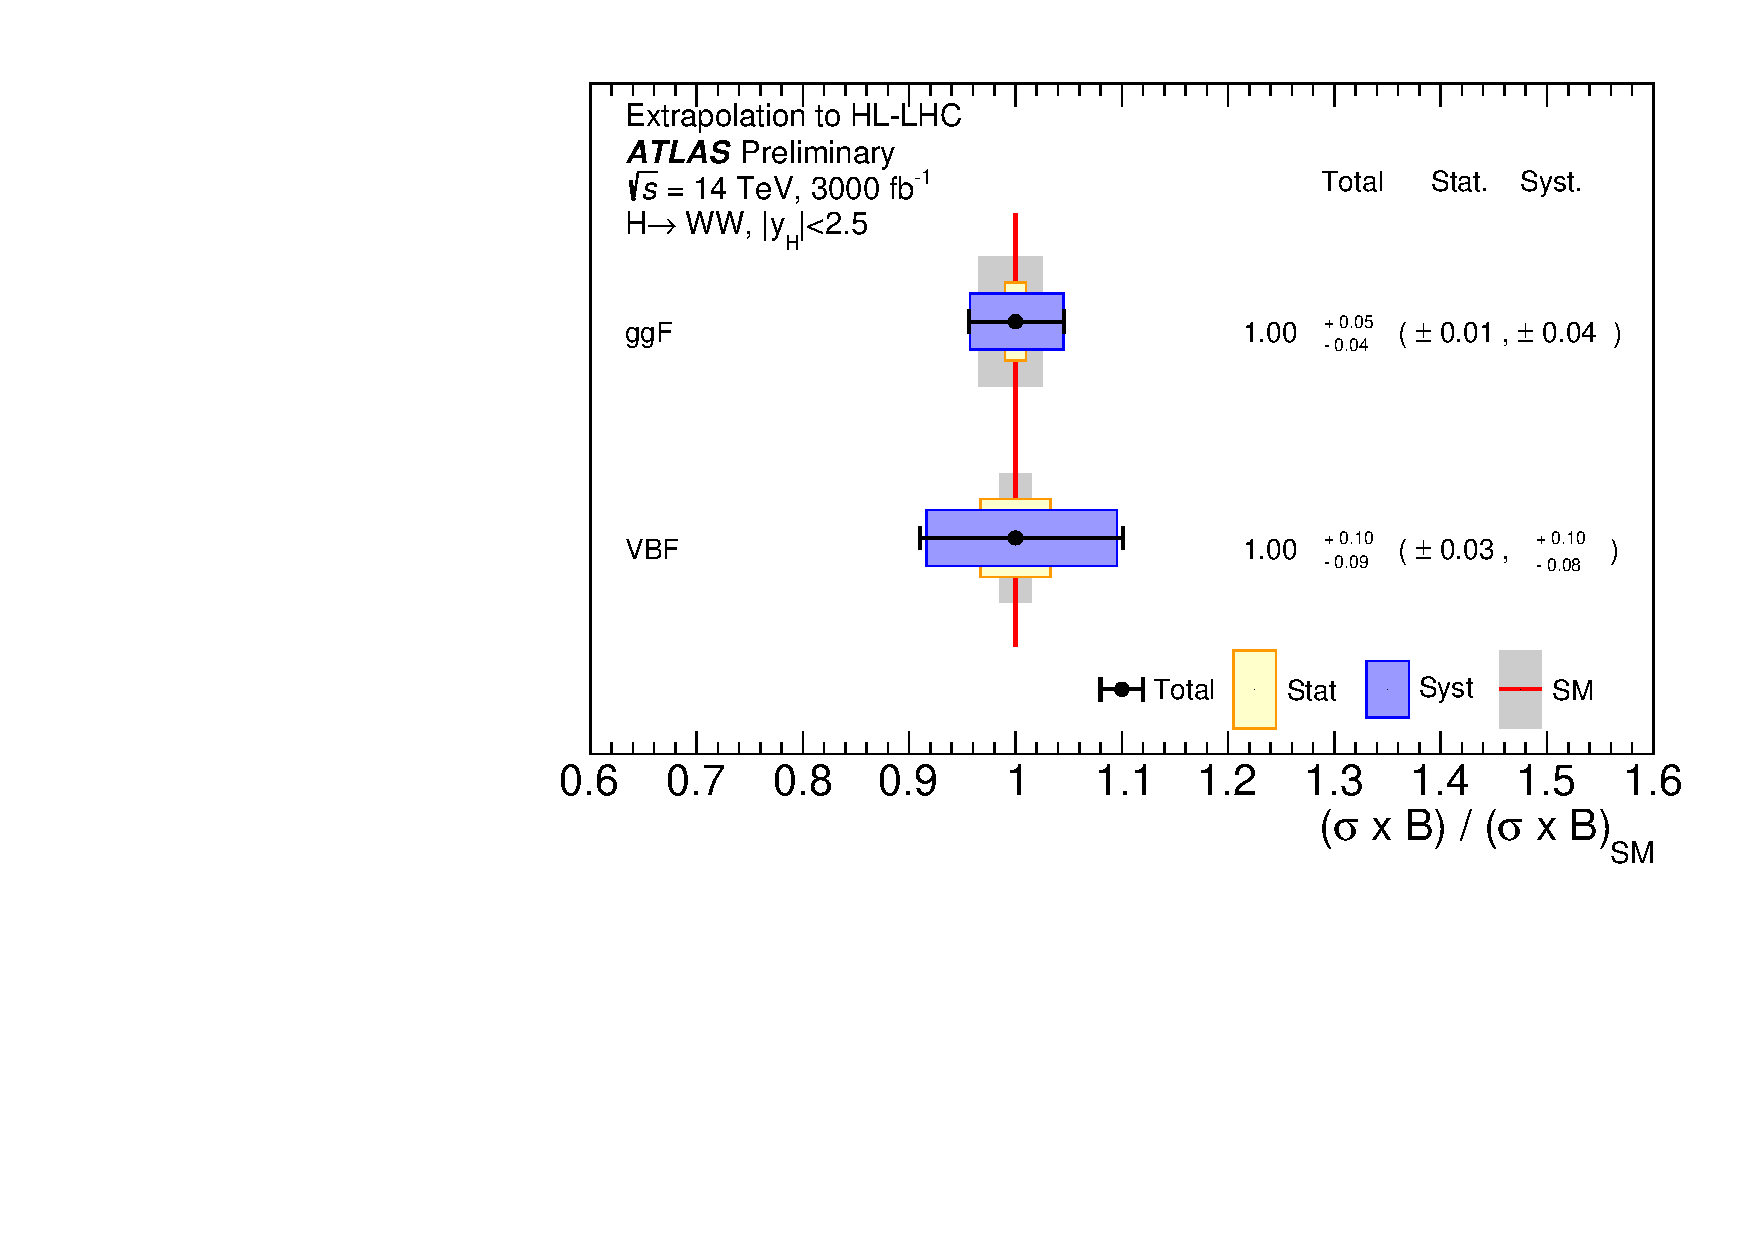
\includegraphics[width=0.56\linewidth]{\main/section2/plots/channels/ATLAS_plot_compareToSM_WW_prodXS}
  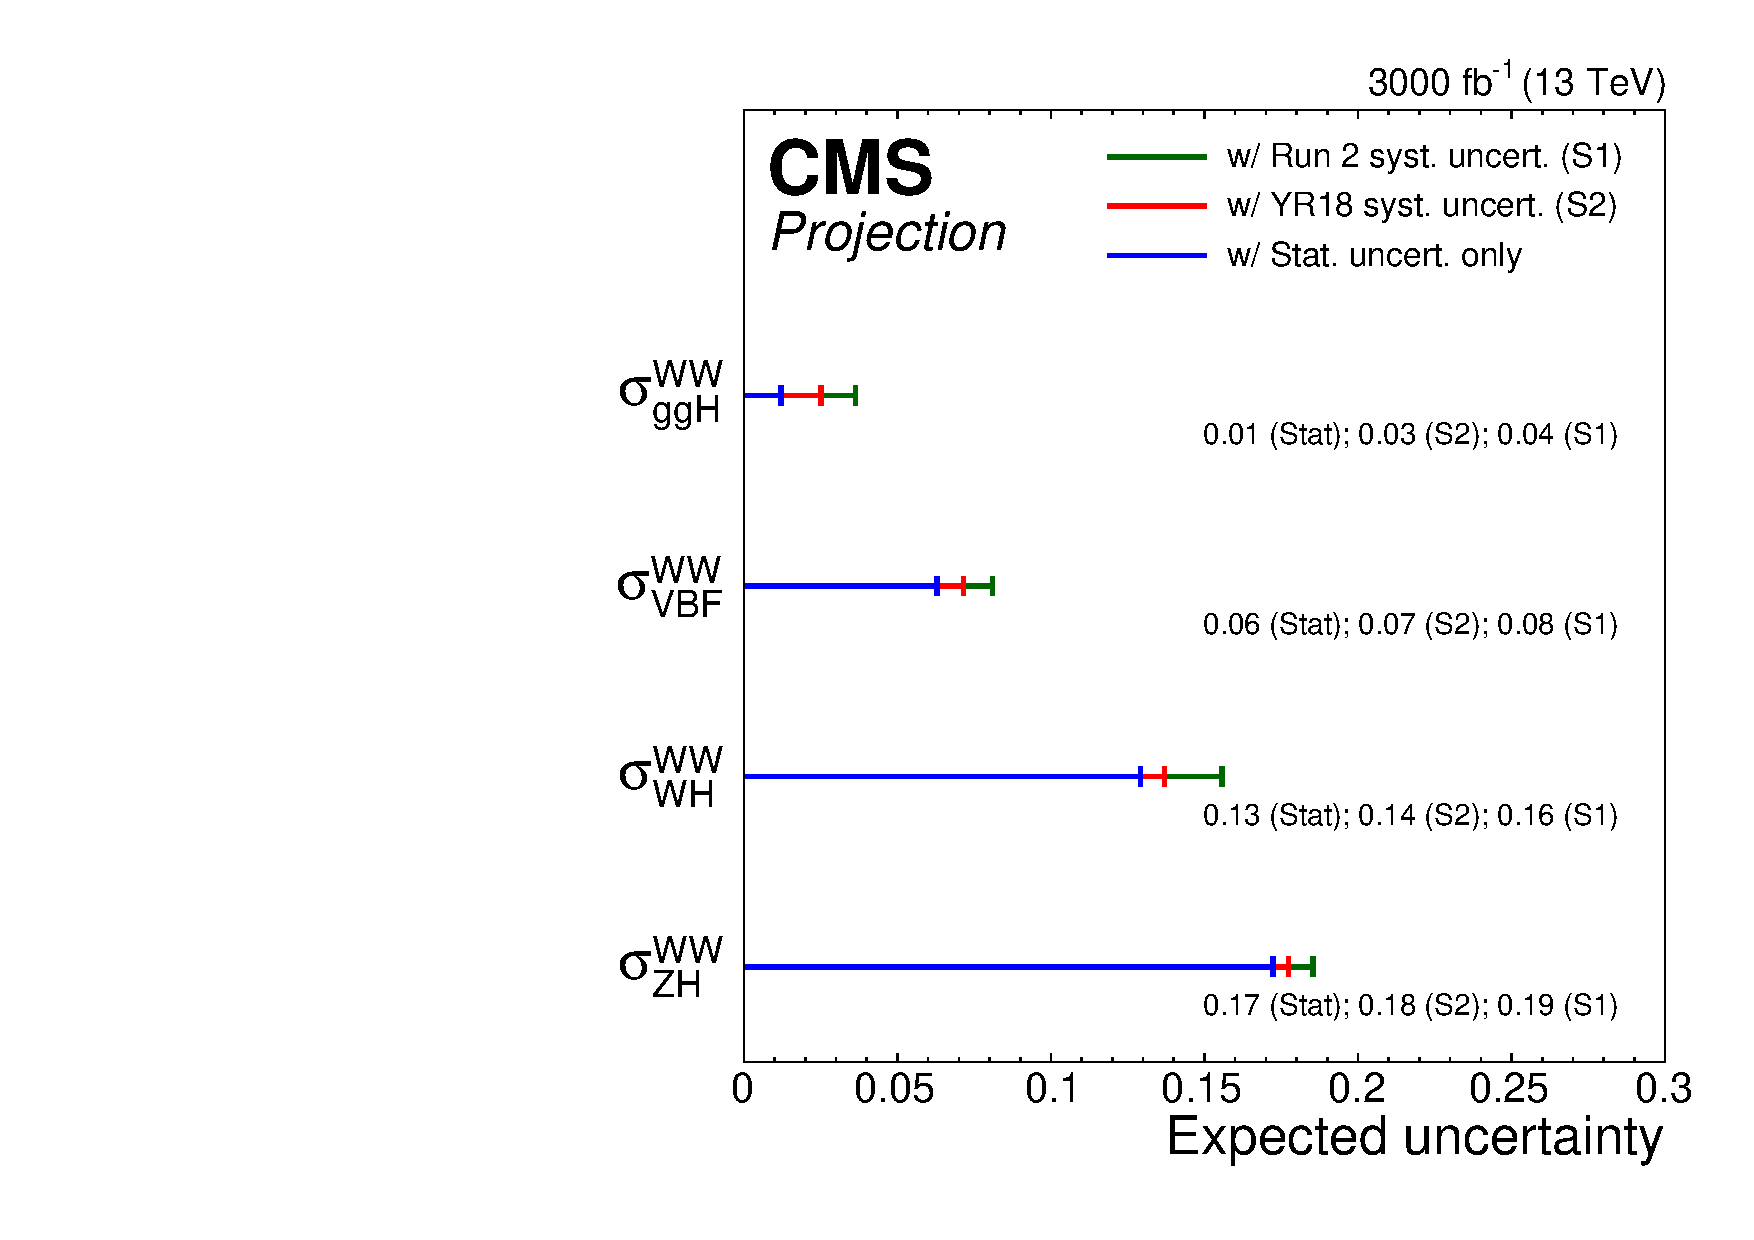
\includegraphics[width=0.42\linewidth]{\main/section2/plots/channels/CMS_summary_A1_5PD_3000_hww}
  \caption{Cross-section times branching fraction measurements of the main Higgs production modes in the \HWW\ decay channel, as extrapolated at the HL-LHC. In case of ATLAS results (left) the ratios of cross sections to their respective theoretical SM predictions are shown for scenario S2, while in case of CMS results (right) the uncertainties on these measurements are shown for S1, S2, and Stat-only scenarios.}
  \label{fig:HWW_ATLAS_HLLHC_S2}
\end{figure}
